\documentclass[PICOReport.tex]{subfiles}

\begin{document}

{\bf Inflation and Gravitational waves} \\ %[0.3cm] 
\comor{add citations to the text?}
Measurements of the \ac{CMB} together with Einstein's theory of general relativity imply that the 
observed density perturbations must have been created long before the \ac{CMB} was released, 
and rather remarkably even before the universe became filled with a hot and dense plasma of 
fundamental particles. The mechanism generating these perturbations, 
which evolved to fill the Universe with structures, is one of the most compelling open questions 
in cosmology.

While the dynamics of the plasma produces some amount of gravitational waves, the amplitude 
is predicted to be too small to be detected in existing or planned experiments. 
Therefore any imprint of gravitational waves on the \ac{CMB} detected by PICO would constitute 
evidence for gravitational waves from the same primordial period that created the density perturbations. 
\comor{the connection with gravitational waves is not completely clear } 
Because the dynamics of gravitational waves is essentially unaffected by the plasma physics, 
they would be a pristine relic left over from the earliest moments of our universe, and their properties 
would shed light on the mechanism that created the primordial perturbations. 
% that grew into the anisotropies of the CMB and the stars and galaxies around us. 
Knowledge of the strength of the 
signal and its statistical properties would transform our understanding of many areas of fundamental physics. 

Inflation, a period of nearly exponential expansion of the early universe, is the leading paradigm 
explaining the origin of the primordial density perturbations. It predicts a nearly scale invariant 
spectrum of primordial gravitational waves originating from quantum fluctuations. Thus, a detection 
of these gravitational waves would be the first detection of phenomenon associated with 
quantum gravity. Because the spectrum is scale-invariant, one may hope to detect primordial 
gravitational waves over a wide range of frequencies including, for example, at LIGO or LISA frequencies. 
However, as a consequence of the expansion of the universe, the energy density in the gravitational 
waves rapidly dilutes with increasing frequency, and observations of the CMB provide the easiest, 
and for the foreseeable future only way to detect these gravitational waves. 

The strength of the signal, often quantified by the tensor-to-scalar ratio $r$, is a direct measure of 
the expansion rate of the universe during inflation. Together with the Friedmann equation, this reveals 
one of the most important characteristics of inflation, its energy scale. PICO will be able to 
detect primordial gravitational waves if inflation occurred at an energy scale of at 
least $4\times 10^{15}\,\rm{GeV}$. \comor{also quote an $r$ value so as to connect to 
the introduction and current limits} A detection would have profound implications for fundamental 
physics because it would provide evidence for a new energy scale, and would allow us to probe 
physics at energies far beyond the reach of terrestrial colliders.

\begin{figure}[!htb]
\centering
\hspace{-0.15in}
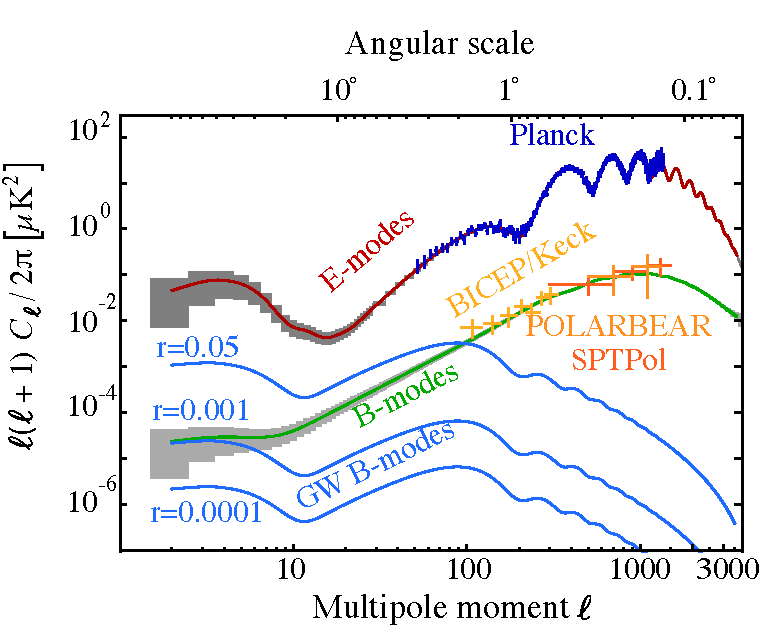
\includegraphics[width=3in]{images/cmb_powspec_PICOv2.pdf}
\hspace{-0.15in}
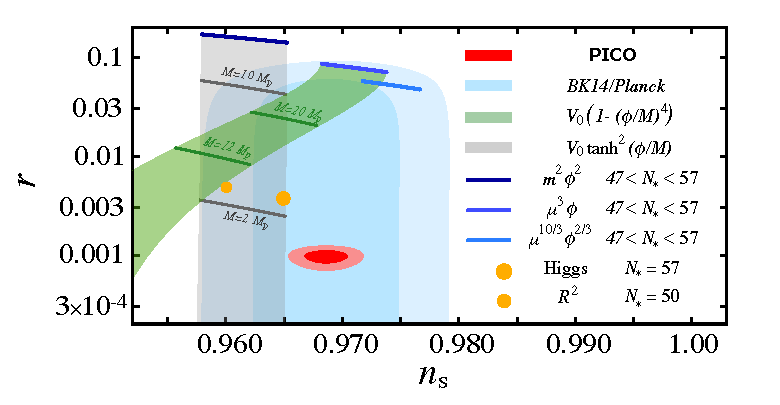
\includegraphics[width=3.6in]{images/nsrlabeledrp001_PICOv1.pdf}
\caption{Predicted $1\sigma$ errors (grey) for determining the E (red) and B-mode (green) angular power 
spectra by PICO for an Inflationary gravity wave B-mode with $r=0.001$. \comor{use r=5e-4? 
need to extend error bars to show high $\ell$ limit.}  Also shown are power spectra 
for other values (Solid blue), lensing B-mode detection from current experiments, 
and \planck~measurements of the E mode.  
\comor{add noise, separate lensing + label, foregrounds?} }
\label{fig:clbb}
\end{figure}

The signal has two contributions, one on degree angular scales or multipoles of $\ell~\sim~80$, 
typically referred to as the recombination peak, and another contribution for multipoles of $\ell\lesssim 20$ 
from the epoch of reionization; see the left panel of Figure~\ref{fig:clbb}. The contribution from reionization 
is expected 
to be strongest relative to the contributions from instrumental noise and `lensing' (see Section~\ref{??}). \comor{refer to
where ever we talk about lensing. best 
illustrated with a figure. should we add the noise and lensing lines to Figure 1?} 
No sub-orbital experiment has yet measured modes at $\ell<40$. The temporal stability, absence of 
atmospheric noise, and full sky coverage offered by a satellite like PICO make it
the most suitable instrument to reach these lowest multipoles.  

There are two classes of slow-roll inflation that naturally explain the observed value of the 
spectral index of primordial fluctuations $n_s$. The first class is characterized by potentials of the 
form $V(\phi)\propto\phi^p$. This class includes many of of the simplest models of inflation, 
some of which have already been strongly disfavored by existing observations; see the right panel of 
Figure~\ref{fig:clbb}. If the constraints on the spectral index tighten by about a factor 2 with the 
central value unchanged, and the upper limits on $r$ improve by an order of magnitude, this class 
would be ruled out. \comor{complete the argument about PICOs performance?}

The second class is characterized by potentials that exponentially approach a plateau \comor{not
clear which plateau} and include $R^2$ inflation. This model predicts a tensor-to-scalar ratio 
of $r\sim 0.003$. All models in this class with a characteristic scale in the potential that is larger 
than the Planck scale predict a tensor-to-scalar ratio
of $r\gtrsim 0.001$, \comor{are there models in the class that have a characteristic scale 
smaller than the planck scale? what r do they predict?} and an experiment like CMB-S4 could 
exclude these scenarios. 
However, there are models such as the Goncharov-Linde model with a somewhat smaller 
characteristic scale that predict a tensor-to-scalar ratio of $r\sim 4\times 10^{-4}$. 

In the absence of a detection, PICO would limit the amount of gravitational waves to 
$r<10^{-4}$ at $95\%$ CL. This is stronger than current upper limits by three orders of magnitude, 
and stronger than those expected for the ground-based experiment CMB-S4 by an order of magnitude. 
\comor{we need to mention the challenges of delensing, foregrounds, and systematics, and provide 
a link to these sections.}

Models of inflation, or the early universe more generally \comor{need to phrase differently}, 
differ in their predictions for the scalar spectral index $n_{\rm s}$ and its scale dependence, 
often referred to as the running of the spectral index $n_{\rm run}$. With its high resolution 
and low noise levels, PICO will improve the constraints on $n_{\rm s}$ and $n_{\rm run}$ by a factor 
of about two. In addition, PICO will probe the statistical properties of the primordial fluctuations 
over a wide range of scales with exquisite precision and improve constraints on departures from 
Gaussianity by a factor $2-3$.

%%%%%%%%%%%%%%%%%%%%%%%%%
\vspace{0.1in}
\parindent = 0pt
{\bf Fundamental Particles: Light relics, Dark Matter, and Neutrinos} \\ %[0.3cm]
\parindent = 15pt
%%%%%%%%%%%%%%%%%%%%%%%%%
$\bullet$ {\bf Light Relics} \hspace{0.1in} In the inflationary paradigm, the universe was reheated to temperatures of 
at least 10 MeV and perhaps as 
high as $10^{12}$ GeV.  At these high temperatures, even very weakly interacting or very massive particles, 
such as those arising in extensions of the Standard Model of particle physics, can be produced in large 
abundances~\cite{1979ARNPS..29..313S,Bolz:2000fu}.  As the universe expands and cools, 
the particles fall out of equilibrium, leaving observable signatures in the CMB power spectra. 
Through these effects the CMB is a sensitive probe of neutrino and of other particles' properties.  

% sensitive probe of the fundamental particle content in the Universe
% large abundance, but not large enough to leave present day signatures? or they decay?
% don't like the words 'extensions of ...' suggests very unlikely things. 

One particularly compelling target is the effective number of light relic particle species $\Neff$.
%, also called the effective number of neutrinos. 
The canonical value with three neutrino families is $\Neff = 3.046$. Additional light particles 
%in thermal equilibrium with the Standard model particles at any point in our history, it will 
contribute a change to $\Neff$ of $\Delta \Neff \geq 0.027\,g$ where $g \geq 1$ is the number of 
degrees of freedom of the new particle~\cite{Brust:2013xpv,Baumann:2016wac}.  
This correction to $\Neff$ is a universal function of the decoupling temperature, with the range 
$ 0.07\,g \geq \ \Delta \Neff \geq 0.027\,g$ corresponding to decoupling from lower temperatures shortly after the QCD phase 
transition ($0.07g$) to higher temperatures near reheating $(0.027g)$.  A measurement of $\sigma(\Neff) \sim 0.03$ would 
at least two orders of magnitude higher decoupling temperatures for particles with spin for which $g \geq 7/4$ and will dramatically extend our knowledge of extensions of the Standard Model.

Performance forecasts for $\Neff$ are shown in Figure~\ref{fig:Neff_future}.  The two most important parameters 
for improving constraints are the fraction of sky observed $f_{\rm sky}$ and the noise. Achieving both larger $f_{\rm sky}$ 
and lower noise are strengths of PICO compared to other platforms. 
Our baseline mission would constraint $\Delta \Neff < 0.06$ at 95\%.  This large improvement over Planck ($\Delta \Neff < 0.28$ at 95\%) would correspond a factor of 200 improvement in the limit on the deccoupling temperture for any particle with spin.  Constraints on $\Neff$ in PICO are largely driven by the TE and EE spectra which are expected to be measured over large fractions of the sky.  This target is achievable with PICO because the the larger sky fraction available from space compensates for the lower resolution required.


\begin{figure}[t!]
\begin{center}
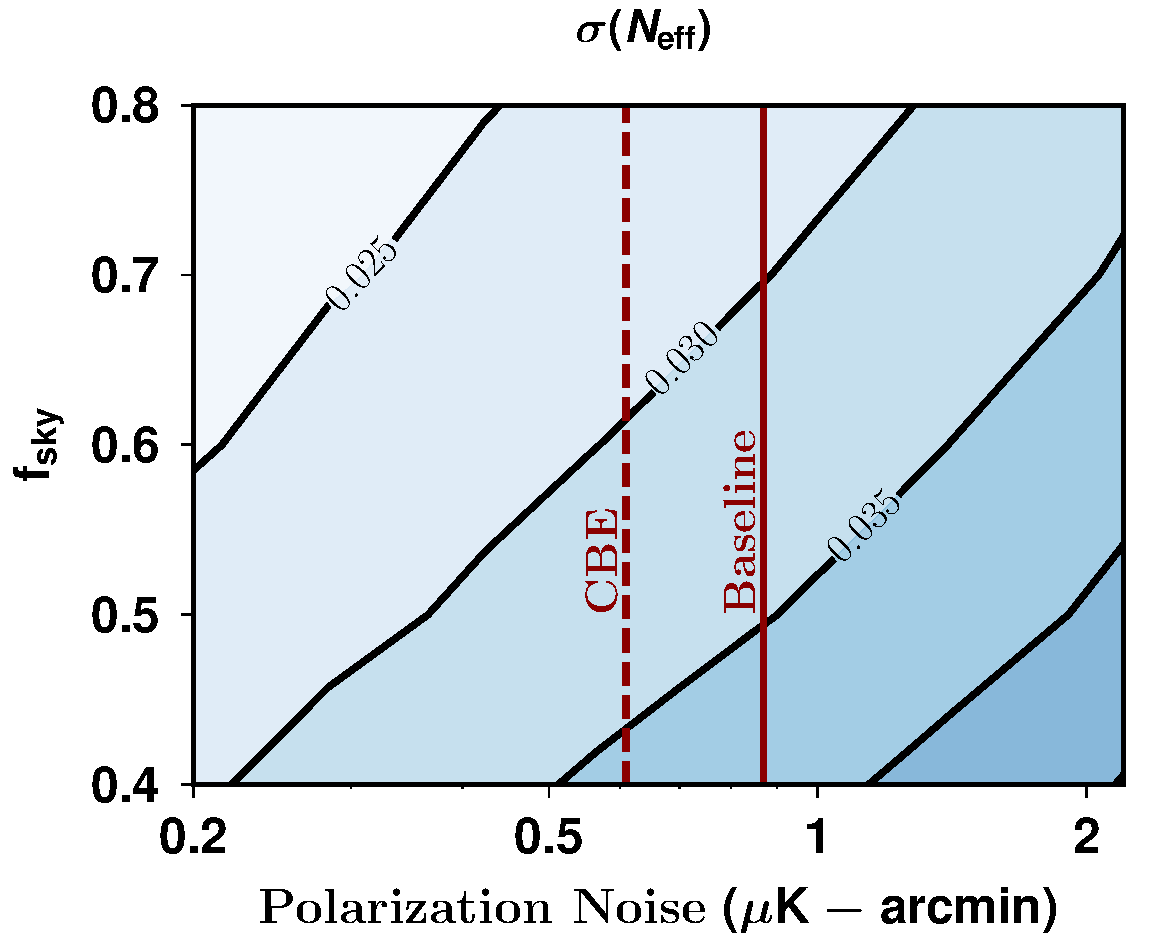
\includegraphics[width=0.45\textwidth]{images/Neff_final.pdf}
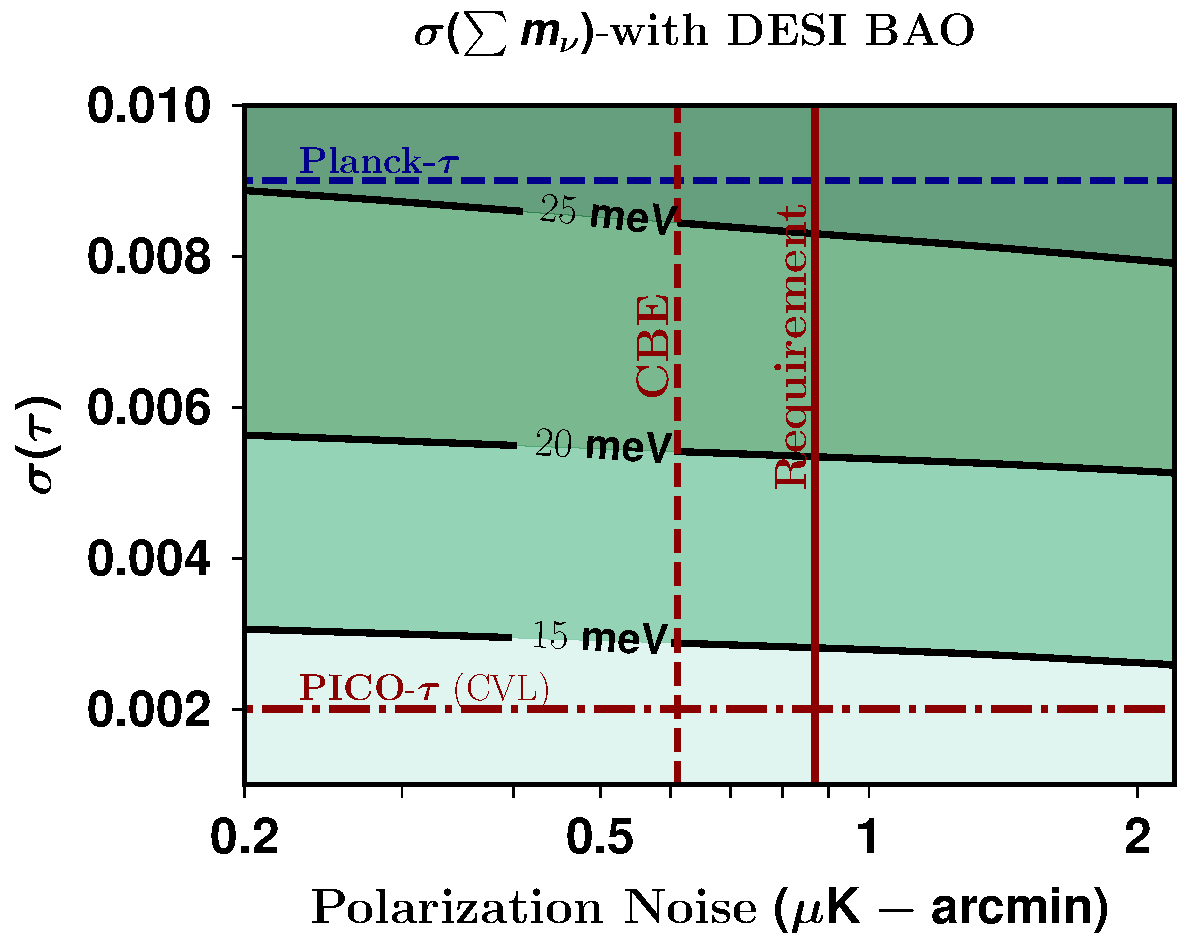
\includegraphics[width=0.47\textwidth]{images/Mnu_tauprior_final.pdf}
\vspace{-0.15in}
\caption{ \small \setlength{\baselineskip}{0.95\baselineskip}
$\Neff$ uncertainty as a function of noise and sky fraction (left) and sum of 
neutrino masses uncertainty as a function of noise and the uncertainty in the measurement of $\tau$, 
for 0.7 sky fraction (right). The resolution assumed is 5'.  
Vertical lines denote the expected performance of the baseline mission. 
The upper blue dashed line is the current \planck~limit; the lower grey dashed line is the limit from cosmic variance 
limited measurement of $\tau$. All forecasts assume internal delensing of the $T$ and $E$-maps~\cite{Green:2016cjr}, 
including residual non-Gaussian covariances.  The $\sum m_\nu$ forecasts include DESI BAO.  
\label{fig:Neff_future} }
\end{center}
\vspace{-0.15in}
\end{figure}

Many light relics of the early universe are not stable. They decay, 
leaving faint evidence of their past existence on other tracers. The relics with sufficiently long lifetime to survive few minutes, 
past the epoch of light element synthesis, leave a signature on the helium fraction $Y_p$.  If they decay 
by the time of recombination, their existence through this period is best measured through the ratio of $\Neff$ to $Y_p$. At both CBE and Requirement sensitivity, this measurement of $Y_p$ improves on the current measurement of $Y_p$ from astrophysical measurements of the primordial helium abundance and will offer a more sensitive window into the physics of BBN or any subsequent deviations from the Standard cosmology. 
 \\
%%%%%
$\bullet$ {\bf Dark Matter} \hspace{0.1in} Cosmological measurements have already confirmed the existence of one relic that 
lies beyond the Standard Model: dark matter. For a conventional WIMP candidate, the CMB places very stringent 
constraints on its properties through the signature of its annihilation on the $T$ and $E$ 
spectra \citep{Peebles2000, Chen2004, Padmanabhan2005}.  Unfortunately, the limits on dark matter annihilation will be saturated by near term measurements~\citep{Madhavacheril:2013cna,}. 

A particle-independent approach is to constrain dark matter interactions that would 
affect the evolution of the effective dark matter fluid and its interactions with baryons or photons.  The simplest example is 
to constrain the baryon-dark matter cross section through its effective coupling of the two fluids~\cite{Dvorkin:2013cea}.  
These couplings affect the evolution of fluctuations and ultimately the $T$ and $E$ spectra. 
The current limits of $\sigma \lesssim 10^{-31}-10^{-34}\,{\rm cm}^2 \times (m_{\rm dm} / {\rm MeV})$ can be 
competitive with direct detection for sub-GeV masses.  
More exotic dark sectors that include long-range forces can produce an even richer phenomenology in the CMB and in the large-scale structure 
without necessarily producing an associated signature in direct detection experiments or 
indirect searches (e.g.~\cite{Cyr-Racine:2013fsa,Buen-Abad:2015ova,Lesgourgues:2015wza}). 
\comor{not clear what this sentence says for PICO? why is DM not in the STM? I think we need a figure} 

A host of other physical phenomena including the existence and properties of axions, primordial magnetic fields, and 
superconducting strings, leave signatures on the spectrum of the CMB and can therefore be constrained by 
the sensitive measurements  of a future Probe (e.g.~\cite{Jedamzik2000, Tashiro2012, Dolgov2013, Tashiro2013, Caldwell2013}).
\comor{not clear how this relates to PICO. do we have forecasts?}\\
 %%%%%
 $\bullet$ {\bf Neutrino Mass} \hspace{0.1in} The origin and structure of the neutrino masses is one of the great outstanding 
 questions about the nature of the Standard Model particles.  Measurements of neutrinos in the lab have revealed much 
 about the mass differences and mixing angles.  Cosmology offers a 
 measurement of the sum of the neutrino masses $\sum m_\nu$ through the gravitational influence of the non-relativistic 
 cosmic neutrinos (confirmed by the measurement of $\Neff$) \comor{not clear, what is confirmed?}.  
 The best current constraint arises from a combination of 
 Planck and BOSS \ac{BAO} giving $\sum m_\nu < 0.12$ eV (95\%) \comor{citation}.

Cosmological measurements are primarily sensitive to the suppression of power on small scales after the neutrinos become 
non-relativistic, which can be measured via CMB lensing or weak lensing in a galaxy survey.  However, these measurements are 
limited by our knowledge of the amplitude of the primordial fluctuation power spectrum, $A_s$.  In practice, CMB observations most 
directly constrain $A_s e^{-2 \tau}$ 
and thus do not provide a high precision measurement of $A_s$ or $\tau$.  

%ONLY CMB NEEDS TAU? I THOUGHT ALL SURVEYS DO?

Although many surveys hope to detect $\sum m_\nu$, any detection 
of the minimum value expected from particle physics $\sum m_\nu = 58$~meV at more than $2 \sigma$ will 
require a better measurement of $\tau$.  The best constraints on $\tau$ come from $E$ modes with $\ell < 20$ which require 
measurements over the largest angular scales. To date, the only proven method for such a measurement is from space. 
The current limit of $\sigma({\tau}) = 0.009$ is from \planck~\cite{planck2016_xlvi} \comor{now 0.007}.  Forecasts for a
CMB measurement of $\sum m_\nu$ using the lensing $B$ mode~\cite{Kaplinghat:2003bh} are shown in 
Figure~\ref{fig:Neff_future}.  With the current uncertainty in $\tau$ one is limited to  
$\sigma(\sum m_\nu) \gtrsim 25$ meV; no other survey or cosmological probe would improve this constraint.  
But PICO will reach the cosmic variance limit of $\tau \sim 0.002$ and will therefore 
reach $\sigma(\sum m_\nu) < 15$ meV when combined with DESI's measurements of 
baryon acoustic oscillations~\cite{Levi:2013gra}.  Robustly detecting neutrino mass at  $> 3\sigma$ in any cosmological setting is 
only possible with an improved measurement of $\tau$ like the one achievable with PICO. The measurement
would give  $\sum m_\nu>0$ at greater than $4\sigma$. \comor{how does this compare to forthcoming measurements 
in the lab?, we should probably remove the next sentence about hierarchy.}

or would exclude the inverted hierarchy ($\sum m_\nu > 100$ meV) at 95\% confidence, depending on the central value of the measurement.


%%%%%%%%%%%%%%%%%%%%%%%%%
\vspace{0.1in}
\parindent = 0pt
{\bf Fundamental Fields: Primordial Magnetic Fields and Cosmic Birefringence} \\ %[0.3cm]
\parindent = 15pt
%%%%%%%%%%%%%%%%%%%%%%%%%
$\bullet$ {\bf Primordial Magnetic Fields} \hspace{0.1in} One of the long standing puzzles in astrophysics is the origin of 1-10~$\mu$G strength galactic magnetic fields~\cite{Widrow:2002ud}. Producing a 1~$\mu$G field through a dynamo mechanism would require a seed field of $\sim$0.1~nG~\cite{Widrow:2011hs}. Moreover, $\mu$G strength fields have been observed in proto-galaxies that are too young to have gone through the number of revolutions necessary for the dynamo to work. A primordial magnetic field (PMF), present at the time of galaxy formation, could provide the seed or even eliminate the need for the dynamo altogether. PMFs could have been generated in the aftermath of phase transitions in the early universe~\cite{Vachaspati:1991nm}, during inflation~\cite{Turner:1987bw,Ratra:1991bn}, or at the end of inflation~\cite{DiazGil:2007dy}. Once produced, they would be sustained by the primordial plasma in a frozen-in configuration until the epoch of recombination and beyond leaving potentially observable imprints in the CMB. Thus, constraints on PMF offer a valuable tool for discriminating among different theories of the early universe physics~\cite{Barnaby:2012tk,Long:2013tha,Durrer:2013pga}. Specifically, constraining the contribution of PMF to below 0.05~nG would rule them out as the source for galactic magnetic fields. \comor{is this the only goal? what level is needed to constrain the other models mentioned earlier?} 

The signature of PMF is detectable through Faraday rotation, which converts $E$ modes into $B$ modes, and through generating signatures in the $BB$ power spectrum at high~\ell~\cite{??} \comor{Levon, can you please put the most relevant references for this sentence?}. 
The current CMB bounds on PMF strength \comor{are these the strongest constraints available? are there constraints by other probes? is the CMB expected to give the strongest constraint in the future?} are $B_{\rm 1Mpc}<2$ nG at 95\% CL after marginalizing over the magnetic spectral index and $B_{\rm 1Mpc}<1.2$ nG for the scale-invariant~PMF spectrum \cite{Zucca:2016iur}. 
% derived from a combination of the 2015 Planck TT, EE, TE spectra \cite{Adam:2015rua} and the SPT B-mode spectrum \cite{Keisler:2015hfa}. Without the SPT B-modes, the bounds are considerably weaker: $B_{\rm 1Mpc}<4.4$ nG and $B_{\rm 1Mpc}<2$ nG, respectively \cite{Ade:2015cva,Zucca:2016iur}, demonstrating the importance of B-modes for PMF constraints.



%A stochastic PMF contributes to CMB anisotropies through metric perturbations and the Lorentz force exerted on ions in the pre-recombination plasma \cite{Mack:2001gc,Lewis:2004ef,Finelli:2008xh,Paoletti:2008ck,Shaw:2009nf}. Of particular importance are the vortical perturbations (vector modes) which contribute to the B-mode spectrum \cite{Subramanian:1997gi} on small angular scales  ($l \simeq 2000$) with an amplitude proportional to $B^4_{1\rm{Mpc}}$, where $B_{1\rm{Mpc}}$ is the PMF strength smoothed over one megaparsec. PMF also source gravitational waves (``passive'' tensor modes) which, for a scale-invariant PMF, are indistinguishable from the inflationary gravity wave signal with an amplitude proportional to $B^4_{1\rm{Mpc}} [\ln(a_\nu / a_{\rm{PMF}})]^2$ \cite{Lewis:2004ef}, where $a_\nu$ is the scale factor at neutrino decoupling, and $a_{\rm{PMF}}$ is the scale factor at which PMF was generated. In addition, Faraday rotation (FR) of CMB polarization converts some of the E modes into B modes \cite{Kosowsky:1996yc,Pogosian:2011qv} inducing mode-coupling correlations between E, B and T \cite{Kamionkowski:2008fp,Gluscevic:2009mm,Gluscevic:2012me,Pogosian:2013dya}. Other effects, which are more challenging to model accurately \cite{Chluba:2015lpa}, arise from the dissipation of PMF on small scales, which generates spectral distortions and alters the recombination history \cite{Jedamzik:2013gua,Kunze:2014eka}.

The current CMB bounds on the PMF strength are $B_{\rm 1Mpc}<2$ nG at 95\% CL after marginalizing over the magnetic spectral index and $B_{\rm 1Mpc}<1.2$ nG for the scale-invariant PMF spectrum \cite{Zucca:2016iur}, derived from a combination of the 2015 Planck TT, EE, TE spectra \cite{Adam:2015rua} and the SPT B-mode spectrum \cite{Keisler:2015hfa}. Without the SPT B-modes, the bounds are considerably weaker: $B_{\rm 1Mpc}<4.4$ nG and $B_{\rm 1Mpc}<2$ nG, respectively \cite{Ade:2015cva,Zucca:2016iur}, demonstrating the importance of B-modes for PMF constraints.

The best case 95\% CL bound expected from the PICO B-mode spectrum is $0.5$ nG for a scale-invariant PMF. PICO will be able to measure the B-mode spectrum across the entire range of angular scales, allowing to simultaneously constrain the magnetic amplitude, $B_{1\rm{Mpc}}$, and the epoch of the PMF generation, $a_{\rm{PMF}}$, which is a valuable handle on the early universe physics that is not available today.

Because the magnetic contribution to CMB spectra scales as $B^4_{1\rm{Mpc}}$, an orders of magnitude improvement in the accuracy of the B-mode spectrum would only result in a modest reduction of the bound on $B_{1\rm{Mpc}}$. In contrast, FR scales linearly with $B_{1\rm{Mpc}}$, promising much tighter bounds on the PMF \cite{Pogosian:2018vfr}. At present, such FR-based PMF bounds are not competitive compared to those from CMB spectra, {\it e.g.} the POLARBEAR collaboration obtained $B_{1\rm{Mpc}} < 93$ nG at 95\% CL \cite{Ade:2015cao} based on the analysis of mode-coupling EB correlations in their 150\,GHz map, but they will improve dramatically with the low noise and high resolutions experiments such as PICO.

Our preliminary forecasts show that PICO's sensitivity and resolution would allow to probe PMFs as weak as $0.05$ nG, although imperfect weak lensing subtraction, galactic foregrounds \cite{Oppermann:2011td,De:2013dra,Pogosian:2013dya}, and other systematic effects will likely prevent reducing the bound below $0.1$ nG. It would, nevertheless, be an important improvement which, in particular, would conclusively rule out the purely primordial (no dynamo) origin of galactic magnetic fields.\bibliography{picopmf}

$\bullet$ {\bf Cosmic Birefringence} \hspace{0.1in}
The simplest dynamical way to model late-time acceleration of the Universe is with a slowly-evolving 
scalar field---the quintessence~\cite{Carroll:1998zi}. Such a field generically couples to electromagnetism through a Chern-Simons-like 
term, and causes linear polarization of photons propagating cosmological distances to rotate. 
The effect of rotation of polarization is known as cosmic birefringence~\cite{Carroll:1998zi} and it can convert the primordial E mode into B mode in 
the CMB maps. It thus produces parity-violating TB and EB cross-correlations
\cite{Kamionkowski:2008fp,Gluscevic:2009mm} whose magnitude depends on the statistical properties of the rotation field in the sky. 
Even though there is no theoretical prediction for the size of rotation, if observed, it would be evidence for physics beyond the
standard model and a potential probe of dark-energy microphysics. 
Previous studies used quadratic-estimator formalism to constrain uniform and direction-dependent cosmic birefringence~\cite{Gluscevic:2012me}, 
with the best current upper limit coming from sub-degree scale polarization measurements 
with POLARBEAR~\cite{Ade:2015cao}. 
A promising way to pursue search for cosmic birefringence in the future is measurement of the off-diagonal EB cross correlations using PICO maps.

Fig.~\ref{fig:CB-forecast} shows a projection for
\textit{Planck}, the current best limit from POLARBEAR, and a forecast for PICO 155 
GHz channel (polarization white noise: $1.3$ $\mu$K-arcmin, resolution: $6.2'$, full sky coverage).
PICO promises to deliver a large factor of improvement as compared to the the current constraints. 
%\begin{figure}[h!]
%\centering \includegraphics[width=0.70\textwidth]{images/birefringence-PICO.pdf}
%\caption{The projected noise curves for \textit{Planck} and PICO (XX channel) and the current limit from POLARBEAR for the cosmic-birefringence rotation-angle autocorrelation, reconstructed from the EB correlation.}
%\label{fig:CB-forecast}
%\end{figure}



%One of the last unknowns of the Standard model of particle physics is the absolute mass scale of the neutrinos.  
%While measurements of neutrino oscillations demonstrate the neutrinos have mass, directly measuring the scale of the masses is challenging experimentally.  
%Current measurement of $\Neff$ confirm the existence of a cosmological abundance of neutrinos whose gravitational influence is detectable in the CMB and in large scale structure.  
%Cosmology is uniquely capable of measuring the sum of neutrino masses, $\sum m_\nu$, through the 
%suppression of the growth of structures in the universe on small scales.   However, all cosmological 
%measurements of $\sum m_\nu$ are fundamentally limited by our uncertainty in $\tau$ due to the strong degeneracy 
%between the optical depth to reionization $\tau$ and the amplitude of the primordial perturbation power spectrum
%$A_s$.  


%A detection of $\sum m_\nu$ at this level is not possible with any other existing survey.

%Larger $\sum m_\nu$ gives a larger suppression and the $\sum m_\nu$ can be measured by 
%The \ac{CMB} Probe would be a valuable tool in the quest for a cosmological detection of $\sum m_\nu$.   
%The sensitivity to $\sum m_\nu$ from suppression of power is limited by our knowledge of 
%the primordial amplitude of fluctuations $A_s$, which is strongly degenerate with the optical depth $\tau$.  
%The current limit on $\tau$ from \planck\ of $\sigma({\tau}) = 0.009$~\cite{planck2016_xlvi} limits 
%$\sigma(\sum m_\nu) \gtrsim 25$ meV. Forecasts for an internal 
%CMB measurement of $\sum m_\nu$ via CMB lensing~\cite{Kaplinghat:2003bh} are shown Figure~\ref{fig:Neff_future} but the conclusion is the same for any proposed cosmological probe.
%This lower limit is common to any measurement that depends on the relative suppression.  
%Therefore, a cosmological detection of the minimum value expected from particle physics  
%$\sum m_\nu = 58$~meV at more than $2 \sigma$ will require a better measurement of $\tau$.  

%The \ac{CMB} Probe will reach the cosmic variance limit of $\tau \sim 0.002$ and will therefore 
%reach $\sigma(\sum m_\nu) < 15$ meV when combined with DESI's measurements of 
%baryon acoustic oscillations~\cite{Levi:2013gra}.  
%A detection of $\sum m_\nu$ at this level is not possible with any other existing survey.
%if not accompanied by an improvement to the measurement of $\tau$.


\end{document}

%\begin{figure}[!htb]
%\centering
%
\includegraphics[width=4cm]{images/example}
%\caption{example}
%\label{fig:im_3}
%\end{figure}
